
\section{Distribution of p-values for all correlations tested}
\label{sec:distr-p-values}

\begin{figure}
  (a)\\
  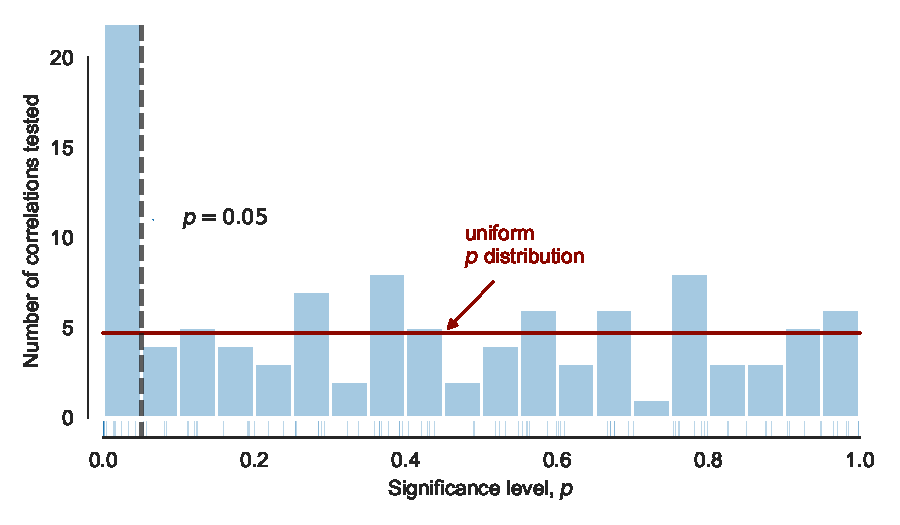
\includegraphics[width=\linewidth]{figs/p-value-histogram-new-linear}\\
  (b)\\
  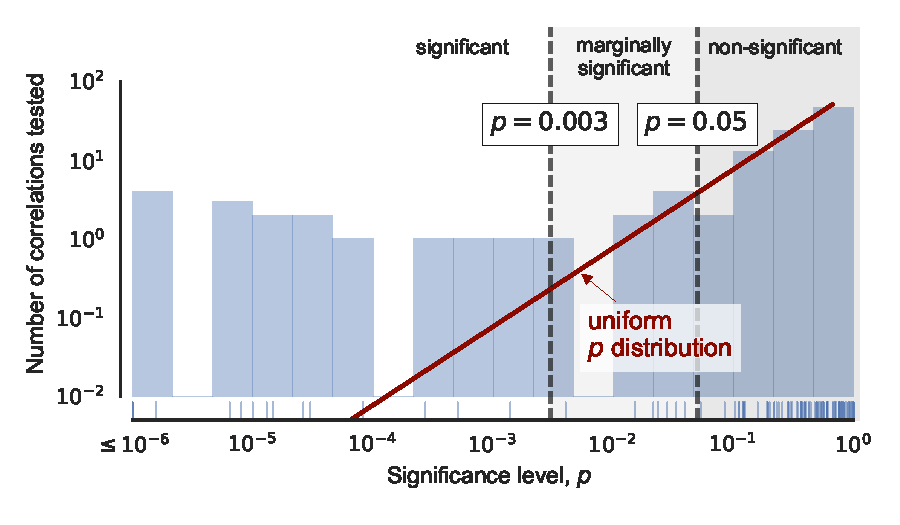
\includegraphics[width=\linewidth]{figs/p-value-histogram-new}
  \caption{Histogram of \(p\)-values for all non-parametric 2-sample
    tests listed in Table~\ref{tab:big-p}. (a)~Uniformly spaced linear
    bins and linear vertical axis. (b)~Uniformly spaced logarithmic
    bins and logarithmic vertical axis, with all values
    \(p \le 10^{-6}\) included in the leftmost bin.  Short thin vertical
    lines above the horizontal axis show the individual value.  The
    thick vertical dashed lines shows the traditional threshold values
    for significance: \(p = 0.003\) (\(\approx 3 \sigma\)) and
    \(p = 0.05\) (\(\approx 2 \sigma\)). The red solid line shows the uniform
    distribution of \(p\)-values that would be expected if the null
    hypothesis were always true, that is, if no significant
    correlations existed.}
  \label{fig:histo-p-values}
\end{figure}

\begin{table*}
  \sisetup{detect-all=true, detect-inline-weight=math}
  \sisetup{round-mode=figures, round-precision=2}
  \sisetup{table-align-exponent = false}
  \setlength\tabcolsep{2pt}
  \caption{Results of all statistical tests performed on observed bow
    shock shape parameters. Significant correlations are shown in
    \textbf{bold}, marginally significant correlations in
    \textit{italic}}
  \label{tab:big-p}
  %%% MIPSGAL summary statistics
%%% Table automatically generated from mipsgal-summary-stats.tab
%%% 2017-06-08 14:17:39.847703
%%%
% \Width is used to align number under col header in first column
	\newlength\Width\settowidth\Width{Comparison}
	\begin{tabular}{@{} ll @{\quad } S[round-mode=places]S[round-mode=places] S[round-mode=places]S[round-mode=places] SS SS @{\quad\quad\quad} SSS[round-mode=places] @{\quad} S@{}S@{}S @{}}\toprule
	  & {Dependent} & \multicolumn{2}{c}{Mean} & \multicolumn{2}{c}{Std.\ Dev.} & \multicolumn{2}{c}{Obs.\ Disp.} & \multicolumn{2}{c @{\quad\quad\quad}}{s.e.m.} & \multicolumn{3}{c @{\quad} }{\dotfill Effect sizes\dotfill } & \multicolumn{3}{c}{\dotfill Non-parametric test \(p\)-values  \dotfill} \\ 
	  {Comparison} & {Variable} & {\(\langle \text{A} \rangle\)} & {\(\langle \text{B} \rangle\)} & {\(\sigma_{\text{A}}\)} & {\(\sigma_{\text{B}}\)} & {\(\langle \epsilon_{\text{A}} \rangle\)} & {\(\langle \epsilon_{\text{B}} \rangle\)} & {\((\sigma/\!\sqrt n)_{\text{A}}\)} & {\((\sigma/\!\sqrt n)_{\text{B}}\)} & {\(r_b\)} & {Cohen \(d\)} & {\(\sigma_{\text{A}}/\sigma_{\text{B}}\)} & \multicolumn{1}{c}{Anderson--Darling} & \multicolumn{1}{c}{Rank biserial} &  \multicolumn{1}{c}{Brown--Forsythe}\\
	  {\makebox[\Width]{(1)}} & \multicolumn{1}{c@{\quad}}{(2)} & {(3)} & {(4)} & {(5)} & {(6)} & {(7)} & {(8)} & {(9)} & {(10)}  & {(11)} & {(12)} & {(13)} & {(14)} & {(15)} & {(16)} \\  
	  \midrule\multicolumn{10}{@{} l @{\quad\quad\quad}}{\itshape Median split of continuous independent variables \dotfill}\\
\addlinespace
Faint/bright & \(R_{90} / R_{0}\) & 1.677 & 1.768 & 0.269 & 0.316 & 0.231 & 0.236 & 0.025 & 0.03 & \itshape 0.174 & \itshape 0.308 & 1.175 & \itshape 0.0215 & \itshape 0.0235 & 0.125\\
\(H\) magnitude & \(\Delta R_{90} / R_{90}\) & 0.183 & 0.198 & 0.161 & 0.163 &   &   & 0.015 & 0.015 & 0.07 & 0.093 & 1.013 & 0.538 & 0.365 & 0.761\\
\(n_{\text{A}} =  n_{\text{B}} = 113\) & \(R_{c} / R_{0}\) & 1.655 & 1.917 & 0.631 & 1.045 & 0.097 & 0.078 & 0.059 & 0.098 & 0.123 & 0.303 & \itshape 1.654 & 0.123 & 0.111 & \itshape 0.0335\\
\addlinespace
Low/high & \(R_{90} / R_{0}\) & 1.707 & 1.739 & 0.25 & 0.336 & 0.256 & 0.212 & 0.024 & 0.031 & 0.061 & 0.11 & \bfseries 1.342 & \itshape 0.0281 & 0.428 & \bfseries 0.00139\\
bow shock size, \(R_0\) & \(\Delta R_{90} / R_{90}\) & 0.175 & 0.204 & 0.157 & 0.165 &   &   & 0.015 & 0.015 & 0.091 & 0.176 & 1.054 & 0.103 & 0.238 & 0.193\\
\(n_{\text{A}} =  n_{\text{B}} = 113\) & \(R_{c} / R_{0}\) & 1.766 & 1.803 & 0.975 & 0.755 & 0.114 & 0.062 & 0.092 & 0.071 & 0.1 & 0.043 & 0.774 & 0.228 & 0.192 & 0.599\\
\addlinespace
Low/high & \(R_{90} / R_{0}\) & 1.703 & 1.742 & 0.267 & 0.323 & 0.233 & 0.235 & 0.025 & 0.03 & 0.04 & 0.132 & 1.213 & 0.554 & 0.602 & 0.123\\
extinction, \(A_K\) & \(\Delta R_{90} / R_{90}\) & 0.186 & 0.195 & 0.138 & 0.183 &   &   & 0.013 & 0.017 & -0.039 & 0.057 & 1.326 & 0.301 & 0.61 & 0.112\\
\(n_{\text{A}} =  n_{\text{B}} = 113\) & \(R_{c} / R_{0}\) & 1.725 & 1.846 & 0.822 & 0.917 & 0.091 & 0.085 & 0.077 & 0.086 & 0.082 & 0.139 & 1.116 & 0.219 & 0.285 & 0.982\\
\addlinespace
Low/high & \(R_{90} / R_{0}\) & 1.722 & 1.724 & 0.328 & 0.261 & 0.234 & 0.234 & 0.031 & 0.024 & 0.02 & 0.008 & 0.796 & 0.308 & 0.795 & 0.0534\\
\(\vert{}b\vert\) & \(\Delta R_{90} / R_{90}\) & 0.188 & 0.191 & 0.161 & 0.162 &   &   & 0.015 & 0.015 & 0.009 & 0.021 & 1.005 & 0.964 & 0.907 & 0.694\\
\(n_{\text{A}} =  n_{\text{B}} = 113\) & \(R_{c} / R_{0}\) & 1.706 & 1.862 & 0.727 & 0.988 & 0.085 & 0.091 & 0.068 & 0.092 & 0.069 & 0.181 & 1.358 & 0.19 & 0.368 & 0.0842\\
\addlinespace
High/low & \(R_{90} / R_{0}\) & 1.734 & 1.707 & 0.279 & 0.321 & 0.241 & 0.223 & 0.024 & 0.034 & -0.049 & -0.093 & 1.152 & 0.361 & 0.532 & 0.159\\
\(\cos \ell\) & \(\Delta R_{90} / R_{90}\) & 0.182 & 0.201 & 0.155 & 0.171 &   &   & 0.013 & 0.018 & 0.054 & 0.122 & 1.1 & 0.604 & 0.491 & 0.365\\
\(n_{\text{A}}, n_{\text{B}} = 137, 90\) & \(R_{c} / R_{0}\) & 1.807 & 1.751 & 0.946 & 0.742 & 0.09 & 0.084 & 0.081 & 0.078 & -0.0 & -0.064 & 0.785 & 1.03 & 0.999 & 0.549\\
\midrule
\multicolumn{10}{@{} l @{\quad\quad\quad}}{\itshape Categorical independent variables \dotfill}\\
\addlinespace
Environment: & \(R_{90} / R_{0}\) & 1.735 & 1.693 & 0.283 & 0.338 & 0.238 & 0.218 & 0.022 & 0.053 & -0.07 & -0.142 & 1.194 & 0.603 & 0.49 & 0.392\\
Isolated vs Facing & \(\Delta R_{90} / R_{90}\) & 0.19 & 0.195 & 0.161 & 0.172 &   &   & 0.012 & 0.027 & -0.019 & 0.034 & 1.066 & 0.507 & 0.85 & 0.438\\
\(n_{\text{A}}, n_{\text{B}} = 170, 41\) & \(R_{c} / R_{0}\) & 1.757 & 1.852 & 0.854 & 0.899 & 0.087 & 0.083 & 0.066 & 0.14 & 0.042 & 0.11 & 1.053 & 0.713 & 0.676 & 0.377\\
\addlinespace
Environment: & \(R_{90} / R_{0}\) & 1.735 & 1.68 & 0.283 & 0.309 & 0.238 & 0.233 & 0.022 & 0.077 & -0.13 & -0.193 & 1.092 & 0.518 & 0.391 & 0.782\\
Isolated vs \hii & \(\Delta R_{90} / R_{90}\) & 0.19 & 0.175 & 0.161 & 0.138 &   &   & 0.012 & 0.034 & -0.048 & -0.095 & 0.855 & 0.932 & 0.754 & 0.799\\
\(n_{\text{A}}, n_{\text{B}} = 170, 16\) & \(R_{c} / R_{0}\) & 1.757 & 1.907 & 0.854 & 0.955 & 0.087 & 0.105 & 0.066 & 0.239 & 0.024 & 0.174 & 1.118 & 0.496 & 0.875 & 0.255\\
\addlinespace
Single/multiple & \(R_{90} / R_{0}\) & 1.709 & 1.762 & 0.289 & 0.315 & 0.23 & 0.243 & 0.022 & 0.041 & 0.074 & 0.177 & 1.09 & 0.342 & 0.396 & 0.338\\
source candidate & \(\Delta R_{90} / R_{90}\) & 0.184 & 0.206 & 0.162 & 0.16 &   &   & 0.013 & 0.021 & 0.093 & 0.136 & 0.987 & 0.421 & 0.284 & 0.97\\
\(n_{\text{A}}, n_{\text{B}} = 167, 60\) & \(R_{c} / R_{0}\) & 1.767 & 1.833 & 0.825 & 0.988 & 0.09 & 0.08 & 0.064 & 0.128 & 0.027 & 0.076 & 1.198 & 0.999 & 0.756 & 0.605\\
\addlinespace
With/without & \(R_{90} / R_{0}\) & 1.734 & 1.721 & 0.289 & 0.298 & 0.223 & 0.237 & 0.043 & 0.022 & -0.042 & -0.044 & 1.031 & 0.595 & 0.667 & 0.563\\
\SI{8}{\um} emission & \(\Delta R_{90} / R_{90}\) & 0.203 & 0.186 & 0.205 & 0.149 &   &   & 0.031 & 0.011 & 0.021 & -0.106 & 0.726 & 0.765 & 0.826 & 0.219\\
\(n_{\text{A}}, n_{\text{B}} = 45, 182\) & \(R_{c} / R_{0}\) & 1.714 & 1.802 & 0.598 & 0.926 & 0.091 & 0.087 & 0.089 & 0.069 & -0.012 & 0.101 & 1.547 & 0.824 & 0.904 & 0.2\\
\addlinespace
3-star vs (4+5)-star & \(R_{90} / R_{0}\) & 1.661 & 1.812 & 0.288 & 0.286 & 0.247 & 0.216 & 0.025 & 0.029 & \bfseries 0.328 & \bfseries 0.525 & 0.99 & \bfseries 8.23e-05 & \bfseries 2.63e-05 & 0.403\\
 & \(\Delta R_{90} / R_{90}\) & 0.189 & 0.19 & 0.162 & 0.161 &   &   & 0.014 & 0.017 & -0.007 & 0.009 & 0.994 & 0.809 & 0.927 & 0.561\\
\(n_{\text{A}}, n_{\text{B}} = 133, 94\) & \(R_{c} / R_{0}\) & 1.632 & 2.0 & 0.91 & 0.764 & 0.106 & 0.061 & 0.079 & 0.079 & \bfseries 0.386 & \bfseries 0.431 & 0.84 & \bfseries 1.47e-05 & \bfseries 7.66e-07 & 0.762\\
\midrule
\multicolumn{10}{@{} l @{\quad\quad\quad}}{\itshape Intercomparison with other datasets \dotfill}\\
\addlinespace
MIPS vs Orion & \(R_{90} / R_{0}\) & 1.723 & 2.418 & 0.297 & 0.811 &   &   & 0.02 & 0.191 & \bfseries 0.7 & \bfseries 1.928 & \bfseries 2.735 & \bfseries 8.02e-06 & \bfseries 7.84e-07 & \bfseries 6.41e-06\\
 & \(\Delta R_{90} / R_{90}\) & 0.19 & 0.701 & 0.162 & 0.532 &   &   & 0.011 & 0.148 & \bfseries 0.689 & \bfseries 2.553 & \bfseries 3.29 & \bfseries 9.94e-06 & \bfseries 3e-05 & \bfseries 2.42e-10\\
\(n_{\text{A}}, n_{\text{B}} = 227, 18\) & \(R_{c} / R_{0}\) & 1.784 & 2.639 & 0.871 & 1.302 &   &   & 0.058 & 0.307 & \bfseries 0.516 & \bfseries 0.94 & 1.495 & \bfseries 0.000505 & \bfseries 0.000273 & 0.12\\
\addlinespace
MIPS vs RSG & \(R_{90} / R_{0}\) & 1.723 & 1.402 & 0.297 & 0.092 &   &   & 0.02 & 0.035 & \bfseries -0.742 & \bfseries -1.098 & \itshape 0.311 & \bfseries 0.000571 & \bfseries 0.000841 & \itshape 0.0406\\
 & \(\Delta R_{90} / R_{90}\) & 0.19 & 0.15 & 0.162 & 0.087 &   &   & 0.011 & 0.033 & -0.072 & -0.247 & 0.539 & 0.795 & 0.747 & 0.286\\
\(n_{\text{A}}, n_{\text{B}} = 227, 7\) & \(R_{c} / R_{0}\) & 1.784 & 1.437 & 0.871 & 0.083 &   &   & 0.058 & 0.031 & -0.191 & -0.405 & 0.095 & 0.0798 & 0.392 & 0.053
\\
\bottomrule
\end{tabular}

\end{table*}

Results from all the statistical tests discussed in
\S~\ref{sec:corr-shape} are given in Table~\ref{tab:big-p}.


% \begin{table}
%   \caption{Lower bounds on the Type~I error rate, \(\alpha\)}
%   \label{tab:type-I}
%   \centering
%   \begin{tabular}{lrr} \toprule
%     Correlation & \(p\) & \(\alpha\) \\
%     \midrule
%     \multicolumn{3}{l}{\itshape Quantitative \dotfill}\\
%     \(R_c\) vs \(R_0\) & \textit{0.0054} & \textit{0.0712} \\
%     \(R_{90}\) vs \(R_0\) & \textbf{0.0001} & \textbf{0.0025} \\
%     \(R_c\) vs \(H_0\) & 0.1229 & 0.4119 \\
%     \(R_{90}\) vs \(H_0\) & \textit{0.0215} & \textit{0.1833} \\
%     \(R_c\) vs \(A_K\) & 0.19 & 0.4617 \\
%     \(R_{90}\) vs \(A_K\) & 0.63 & 1 \\
%     \(R_c\) vs \(|b|\) & 0.19 & 0.4617 \\
%     \(R_{90}\) vs \(|b|\) & 0.31 & 0.4967 \\
%     \(R_c\) vs \(\cos(\ell)\) & 1.00 & 1 \\
%     \(R_{90}\) vs \(\cos(\ell)\) & 0.36 & 0.4999 \\
%     \midrule
%     \multicolumn{3}{l}{\itshape Categorical} \dotfill\\
%     \(R_c\) vs Facing & 0.71 & 1 \\
%     \(R_c\) vs H II & 0.50 & 1 \\
%     \(R_{90}\) vs Facing & 0.60 & 1 \\
%     \(R_{90}\) vs H II & 0.52 & 1 \\
%     \(R_c\) vs Multiple & 1.00 & 1 \\
%     \(R_{90}\) vs Multiple & 0.34 & 0.4993 \\
%     \(R_c\) vs \SI{8}{\um} & 0.82 & 1 \\
%     \(R_{90}\) vs \SI{8}{\um} & 0.6 & 1 \\
%     \midrule
%     \multicolumn{3}{l}{\itshape Other datasets} \dotfill\\
%     \(R_c\) vs Herschel & 0.074 & 0.3437 \\
%     \(R_{90}\) vs Herschel & \textbf{0.00052} & \textbf{0.0106} \\
%     \(R_c\) vs M42 & \textbf{0.00048} & \textbf{0.0099} \\
%     \(R_{90}\) vs M42 & \textbf{0.0000105} & \textbf{0.0003} \\
%     \bottomrule
%   \end{tabular}
% \end{table}


The \(p\)-values are the probability of finding a difference between
two populations as large as (or larger than) what is observed,
\emph{given} that there is no difference in the underlying
distribution from which the two populations are drawn (that is, given
that the null hypothesis is true).  However, what we really want to
know is something else: the probability that the null hypothesis is
true, \emph{given} the observations.  That is, the probability,
\(\alpha\), of a \textit{false positive}, also known as the \textit{Type I
  error rate}.  The common mistake of conflating these two definitions
is known as the ``\(p\)-value fallacy'' \citep{Goodman:1999a}, or``the
error of the transposed conditional'', as discussed in detail by
\citet{Colquhoun:2014a}.  It is possible to derive \(\alpha\) from
\(p\) using Bayes' theorem (e.g., \citealp{Goodman:1999b}), but that
requires an estimate of the prior probability of the null hypothesis,
independent of the observations.  Alternatively, it is also possible
to find a lower bound on \(\alpha\) from a frequentist approach
\citep{Sellke:2001a}:
\begin{equation}
  \label{eq:type-I}
  \alpha(p) \ge \bigg[ 1 - \big(e\, p \ln p\big)^{-1} \bigg]^{-1}
  \quad \text{valid for } p < 1/e.
\end{equation}
This is the approach we adopt here, which also numerically coincides
with the Bayesian approach for the case where the prior probability of
the null hypothesis is 0.5.  The reason that this is only a lower
limit for \(\alpha\) is that if we have overwhelming a priori evidence that
the null hypothesis is true (for instance, from previous empirical
studies, or because it follows from a well-supported theory), then a
Bayesian calculation would give a much higher value of \(\alpha\) than
\eqref{eq:type-I} does.  In our case, however, we have no strong
reasons for favoring any of the null hypotheses, so it is reasonable
to assume \(\alpha\) is close to the lower limit given in \eqref{eq:type-I}.

In order to choose a threshold \(p\)-value that counts as a
``significant'' result, one then needs to balance the risks of false
positives against the risks of \textit{false negatives}.  The false
negative probability, \(\beta\), also known as \textit{Type II error
  rate}, is the probability of failing to reject an untrue null
hypothesis.  That is, in the context of this paper, it is the
probability of failing to detect a real difference between two
sub-samples, or a real correlation between two variables.  The
complementary probability, \(1 - \beta\), is known as the
\textit{statistical power} or sensitivity of the test.  The value of
\(\beta\) depends on three factors:
\begin{enumerate}[1.]
\item The \textit{effect size}, which is a measure of the magnitude of
  the difference in a dependent variable between two sub-samples, or
  the degree of correlation between two continuous variables.  For the
  two sub-sample case, it is common to use a standardised mean
  difference, such as Cohen's \(d\) statistic \citep{Cohen:1988a}:
  \(d = (\bar{X}_A - \bar{X}_B) / s\), where \(\bar{X}_A\),
  \(\bar{X}_B\) are the means of the dependent variable \(X\) for
  samples A and B, while \(s\) is the pooled standard deviation of
  \(X\).  For the case of two continuous variables, the Pearson linear
  correlation coefficient, \(r\), can be used.  In both cases, rules
  of thumb have been developed \citep{Ruscio:2008a} for classifying an
  effect as ``large'' (\(d > 0.8\), \(r > 0.4\)) or ``small''
  (\(d < 0.2\), \(r < 0.1\)).  Alternatively, non-parametric
  statistics can be used, such as the \(A\) measure of stochastic
  superiority \citep{Delaney:2002a}.
\end{enumerate}

Obviously, this depends on the \textit{effect size}, which is the 


All astronomical data analysis is \emph{post hoc} analysis, since the universe was not set up to test a particular hypothesis (as far as we know).  It is therefore important to guard against the ``multiple comparisons problem'', whereby seemingly significant correlations are found where none really exist, simply by virtue of the large number of tests that were carried out.

Under the more conservative Holm--Bonferroni method, only comparisons with \(p < 0.001\) would be significant. 

The p-curve \citep{Head:2015a}

% \begin{table}
%   \caption{Results of all statistical tests performed on observed
%     bow shock shape parameters.}
%   \begin{tabular}{p{0.95\linewidth}}
%     \toprule
%     \textit{Description of columns:}
%     (Col.~1)~How the two A/B source sub-samples are defined, also giving the size of each sub-sample, \(n_{\text{A}}\) and~\(n_{\text{B}}\).
%     (Col.~2)~Dependent variable whose distribution is compared between the two sub-samples.
%     (Cols.~3--6)~Mean and standard deviation, \(\sigma\), of the dependent variable for each of the two sub-samples.
%     (Cols.~7--8)~Mean over each sub-sample of the observational dispersion (\(\epsilon\), standard deviation) of radii that contribute to the dependent variable for each individual source, as in steps~\ref{step:R0} and \ref{step:R90} of \S~\ref{sec:autom-trac-fitt}.  Note that in the case of \(R_c\), this is \(\epsilon(R_0)\), and so is not a direct measure of the observational uncertainty in \(R_c\). 
%     (Cols.~9--10)~``Standard error of the mean'' (s.e.m.) of the dependent variable for each of the two sub-samples. 
%     (Cols.~11--13)~Standardized ``effect sizes'', which are dimensionless measures of the difference in the distribution of the dependent variable between the two sub-samples.
%     (Col.~11)~Rank biserial correlation coefficient \citep{Cureton:1956a}, which is obtained by considering all \(n_{\text{A}} n_{\text{B}}\) pair-wise comparisons of the dependent variable between a source in sub-sample~A and a source in sub-sample~B.  It is the difference between the fraction of such comparisons ``won'' by sub-sample~A and those ``won'' by sub-sample~B, and thus may vary between \(-1\) and \(+1\). 
%     (Col.~12)~Cohen's \(d\), which is a dimensionless mean difference: \(d = (\langle \text{A} \rangle - \langle \text{B} \rangle) / \sigma_{\text{pool}} \), where \(\sigma_{\text{pool}} = (n_{\text{A}} \sigma_{\text{A}}^2 + n_{\text{B}} \sigma_{\text{B}}^2)^{1/2} / \sqrt{n_{\text{A}} + n_{\text{B}}}\) is the pooled standard deviation.
%     (Col.~13)~Ratio of standard deviations between the two sub-samples.
%     (Cols.~14--16)~Probabilities (\(p\)-values) of the two sub-samples being as different as observed if they were to be drawn from the same population, according to three different non-parametric tests.
%     (Col.~14)~Anderson--Darling 2-sample test, which is a general test of similarity between two distributions that is designed to retain sensitivity to differences in the tails of the distributions.
%     (Col.~15)~Mann--Whitney--Wilcoxon \(U\) test \citep{Mann:1947a}, which is sensitive to differences in the central value of the distributions.
%     (Col.~16)~Brown--Forsythe test for equality of variance \citep{Brown:1974a}
%     \\
%     \bottomrule
%   \end{tabular}
% \end{table}





\section{Perturbed bows}
\label{sec:perturbed-bows}

\begin{figure*}
  \centering
  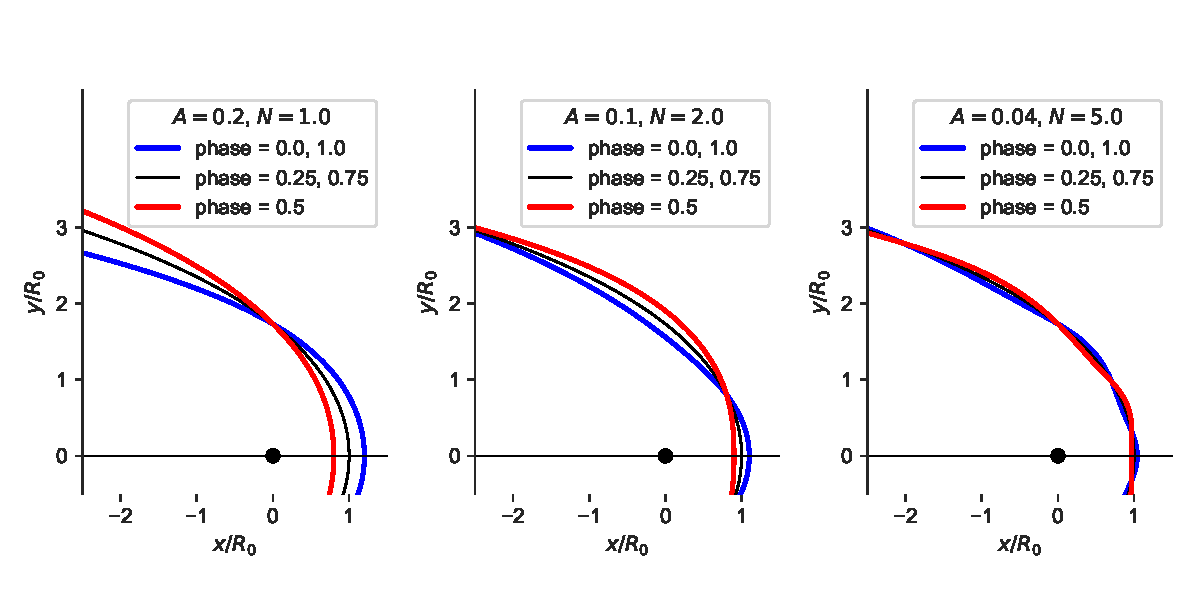
\includegraphics[width=\linewidth]{figs/compare_xyprime_wave-wilkinoid}
  \caption{Small-amplitude standing wave perturbations to wilkinoid
    bow shapes.  The maximum deviations from the base shape are seen
    at phases \(\phi = 0\) (blue line) and \(\phi = 0.5\) (red line), while
    the perturbation is zero at \(\phi = 0.25\) and \(0.75\) (black
    line).  Results are shown left to right for increasing wave
    numbers \(N\) and decreasing amplitudes \(A\): (a)~\(A = 0.2\),
    \(N = 1.0\), (b)~\(A = 0.1\), \(N = 2.0\), (a)~\(A = 0.04\),
    \(N = 5.0\).  The maximum curvature, proportional to \(A N\) is
    the same in all three cases.}
  \label{fig:perturb-shapes}
\end{figure*}
\begin{figure*}
  \centering
  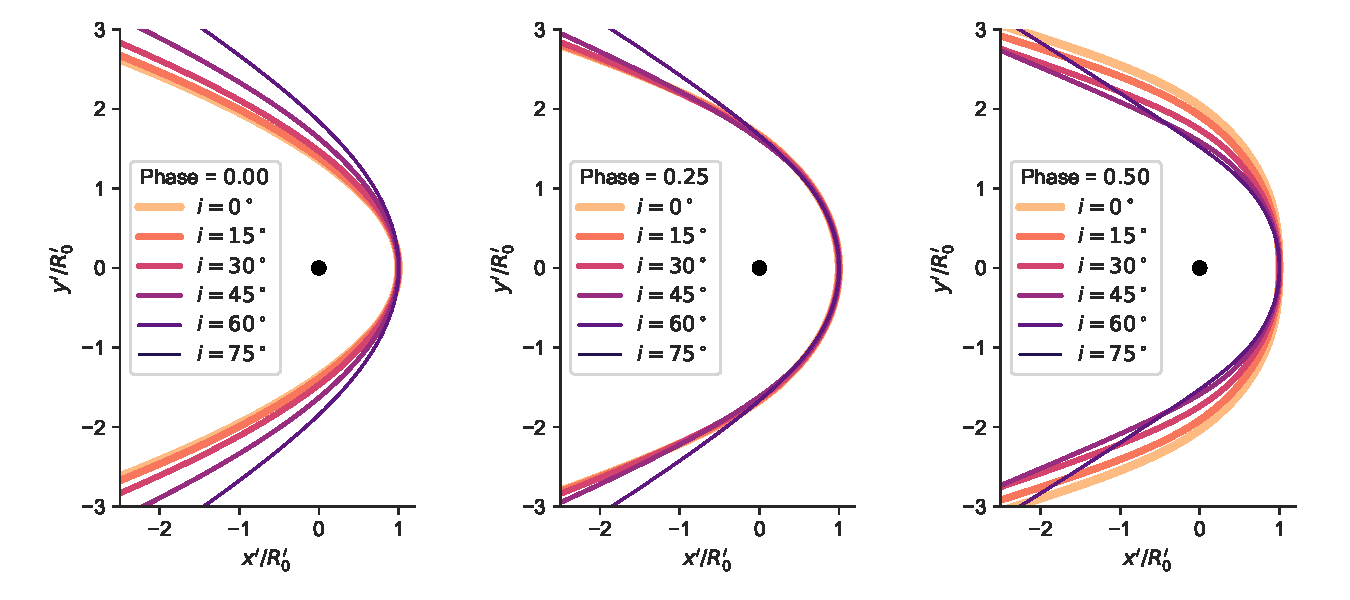
\includegraphics[width=\linewidth]
  {figs/wave_xyprime-A010-N20-ancantoid-xi080-beta000500}
  \caption{Plane-of-sky projections of perturbed bow shapes.  In all
    cases, the base bow shape is ancantoid with \(\xi = 0.8\),
    \(\beta = 0.005\) and the perturbation is the same as in the central
    panel of Fig.~\ref{fig:perturb-shapes}, with amplitude
    \(A = 0.05\) and wave number \(N = 2.0\). Results are shown for
    inclination angles \(i = 0\) to \(i = 75^\circ\) (indicated by line
    color and thickness, see key) and for different fractional phases
    of the oscillation: (a)~\(\varphi = 0.0\), (b)~\(\varphi = 0.25\),
    (c)~\(\varphi = 0.50\). Unlike in Fig.~\ref{fig:perturb-shapes},
    the spatial coordinates are normalized to the instantaneous
    projected apex radius \(R_0'\) at each phase, so the apex does not
    appear to move.}.
  \label{fig:perturb-xy-prime}
\end{figure*}

In this appendix, we present a highly idealized model for small,
time-varying perturbations to a steady-state bow shock shape, such as
those discussed in \S~5 of Paper~0.  These perturbations may be due to
periodic variations in the momentum-loss rate of one of the winds, or
due to dynamical instabilities in the shocked shell.

We consider fractional perturbations \(\Delta(\theta, t)\) of a base shape
\(R(\theta)\), such that
\(R(\theta) \to [1 + \Delta(\theta, t)] R(\theta)\).  For simplicity,
\(\Delta(\theta, t)\) is a standing wave of constant amplitude \(A\), which is
periodic in \(\theta\), with wave number \(N\).  In cylindrical symmetry
\(\Delta(\theta, t)\) must be even in \(\theta\), so can be expressed as
\begin{equation}
  \label{eq:standing-wave}
  \Delta(\theta, t) = A \cos(N \theta) \cos(2\pi \varphi) . 
\end{equation}
For waves with period \(P\), the fractional phase \(\varphi\) will
vary with time \(t\) as
\begin{equation}
  \label{eq:fractional-phase}
  \varphi(t) = (\varphi_0 + t/P) \bmod 1.0\ ,
\end{equation}
where \(\varphi_0\) is an arbitrary reference phase.

Example oscillations with wave numbers \(N = 1.0\), \(2.0\), and
\(5.0\) superimposed on a wilkinoid base shape are shown in
Figure~\ref{fig:perturb-shapes}.  There are \(N\) nodes of the
oscillation between \(\theta = [0, \pi]\), always with an antinode at the apex
(\(\theta = 0\)), as required by symmetry.  So, with \(N = 1.0\) there is a
node (fixed point) in the near wing at \(\theta = \pi/2\), but an antinode in
the far wing at \(\theta = \pi\), which is in antiphase with the oscillation
of the apex, giving rise to a large-scale ``breathing'' mode of
oscillation.  With \(N = 2.0\), there are nodes at \(\theta = \pi/4\) and
\(3\pi/4\), while the antiphase antinode has moved to the near wing at
\(\theta = \pi/2\).  There is still an antinode in the far wing at
\(\theta = \pi\) but it is now in phase with the apex, giving rise to a
``curling-up/straightening-out'' mode of oscillation.  With
\(N = 5.0\), there are many more nodes and antinodes, giving a
``ringing'' mode of oscillation.  Note that all our examples have
\(A \propto 1/N\) in order to keep the local curvature relatively low.  If
the product \(A N\) is not small compared to unity, then the local
curvature can be so extreme as to reverse the concave shape of the
base bow shape, producing locally convex regions.

If the bow shape is viewed at different inclinations, then the effect
of the oscillations on the projected shape will vary.  In particular,
the apex-to-wing interval in body-frame angle changes from
\(\theta = [0, \pi/2]\) at \(i = 0\) to
\(\theta = [\theta_0, \theta_{90}]\) for general \(i\), see equations~(18) and (21)
of Paper~0.  The difference \(\theta_{90} - \theta_0\) is always a declining
function of \(|i|\), so the oscillations of the tangent line become
increasingly stretched out as the inclination increases.  This effect
can be seen in Figure~\ref{fig:perturb-xy-prime}, which shows an
example of the variation in projected perturbed shape with inclination
angle for 3 different phases, this time for an ancantoid base shape
and the \(N = 2.0\) perturbation shown in
Figure~\ref{fig:perturb-shapes}b.  The most marked changes with phase
are seen for low inclinations, whereas the changes are smaller,
although still noticeable, for \(|i| \ge 45^\circ\). If \(A N\) exceeds
about 0.5, then the local curvature of the perturbations is so extreme
that multiple tangent lines exist at intermediate inclinations, which
produces the appearance of additional incomplete bright arcs inside
the main arc of the bow.


%%% Local Variables:
%%% mode: latex
%%% TeX-master: "obs-bowshocks"
%%% End:
